\chapter{Limits of Learning} \label{sec:formal}

\chapterquote{Our lives sometimes depend on computers performing as predicted.}{Philip~Emeagwali}


%\chapterimageopt{serious.png}{width=5cm}{Courtesy XKCD}

\begin{learningobjectives}
\item Define ``inductive bias'' and recognize the role of inductive
  bias in learning.
\item Illustrate how regularization trades off between underfitting
  and overfitting.
\item Evaluate whether a use of test data is ``cheating'' or not.
\end{learningobjectives}

\dependencies{None.}

\newthought{Machine learning is a very general} and useful framework, but it is not ``magic'' and will not always work.
In order to better understand when it will and when it will not work, it is useful to formalize the learning problem more.
This will also help us develop debugging strategies for learning algorithms.

\section{Data Generating Distributions}

Our underlying assumption for the majority of this book is that
learning problems are characterized by some unknown probability
distribution $\cD$ over input/output pairs $(x,y) \in \cX \times \cY$.
Suppose that someone \emph{told} you what $\cD$ was.  In particular,
they gave you a Python function \FUN{computeD} that took two inputs,
$x$ and $y$, and returned the probability of that $x,y$ pair under
$\cD$.  If you had access to such a function, classification becomes
simple.  We can define the \concept{Bayes optimal classifier} as the
classifier that, for any test input $\hat x$, simply returns the $\hat
y$ that maximizes \FUN{computeD}$(\hat x, \hat y)$, or, more formally:
%
\begin{equation} \label{eq:prob:bayesopt}
  f\xth{BO}(\hat x) = \arg\max_{\hat y \in \cY} \cD(\hat x, \hat y)
\end{equation}
%
This classifier is optimal in one specific sense: of \emph{all
  possible} classifiers, it achieves the smallest zero/one error.

\begin{theorem}[Bayes Optimal Classifier] \label{thm:prob:bayesopt}
  The Bayes Optimal Classifier $f\xth{BO}$ achieves minimal zero/one
  error of any deterministic classifier.
\end{theorem}

This theorem assumes that you are comparing against
\emph{deterministic} classifiers.  You can actually prove a stronger
result that $f\xth{BO}$ is optimal for randomized classifiers as well,
but the proof is a bit messier.  However, the intuition is the same:
for a given $x$, $f\xth{BO}$ chooses the label with highest
probability, thus \emph{minimizing} the probability that it makes an
error.

\begin{myproof}{\ref{thm:prob:bayesopt}}
  Consider some other classifier $g$ that claims to be better than
  $f\xth{BO}$.  Then, there must be some $x$ on which $g(x) \neq f\xth{BO}(x)$.  Fix
  such an $x$.  Now, the probability that $f\xth{BO}$ makes an error on this
  particular $x$ is $1 - \cD(x, f\xth{BO}(x))$ and the probability
  that $g$ makes an error on this $x$ is $1 - \cD(x, g(x))$.  But
  $f\xth{BO}$ was chosen in such a way to \emph{maximize} $\cD(x,
  f\xth{BO}(x))$, so this \emph{must} be greater than $\cD(x, g(x))$.
  Thus, the probability that $f\xth{BO}$ errs on this particular $x$ is
  smaller than the probability that $g$ errs on it.  This applies to
  any $x$ for which $f\xth{BO}(x) \neq g(x)$ and therefore $f\xth{BO}$ achieves
  smaller zero/one error than any $g$.
\end{myproof}

The \concept{Bayes error rate} (or \concept{Bayes optimal error rate})
is the error rate of the Bayes optimal classifier.  It is the best
error rate you can ever hope to achieve on this classification problem
(under zero/one loss).
%
The take-home message is that if someone gave you access to the data
distribution, forming an \emph{optimal} classifier would be trivial.
Unfortunately, no one gave you this distribution, so we need to
figure out ways of learning the mapping from $x$ to $y$ given only access to a training set \emph{sampled from} $\cD$, rather than $\cD$ itself.

% Unfortunately, no one gave you this distribution, but this analysis
% suggests that good way to build a classifier is to try to
% \emph{estimate} $\cD$.  In other words, you try to learn a
% distribution $\hat \cD$, which you hope to very similar to $\cD$, and
% then use this distribution for classification.  Just as in the
% preceding chapters, you can try to form your estimate of $\cD$ based
% on a finite training set.

% The most direct way that you can attempt to construct such a
% probability distribution is to select a \emph{family} of parametric
% distributions.  For instance, a Gaussian (or Normal) distribution is
% parametric: it's parameters are its mean and covariance.  The job of
% learning is then to infer which parameters are ``best'' as far as the
% observed training data is concerned, as well as whatever inductive
% bias you bring.  A key assumption that you will need to make is that
% the training data you have access to is drawn \concept{independently}
% from $\cD$.  In particular, as you draw examples $(x_1,y_1) \sim \cD$
% then $(x_2,y_2) \sim \cD$ and so on, the $n$th draw $(x_n,y_n)$ is
% drawn from $\cD$ and \emph{does not} otherwise depend on the previous
% $n-1$ samples.  This assumption is usually false, but is also usually
% sufficiently close to being true to be useful.  Together with the
% assumption that all the training data is drawn from the same
% distribution $\cD$ leads to the \concept{i.i.d. assumption} or
% \concept{independently and identically distributed} assumption.  This
% is a key assumption in almost all of machine learning.


\section{Inductive Bias: What We Know Before the Data Arrives}
\MoveNextFigure{-5cm}
\Figure{dt_birdtrain}{Training data for a binary classification problem.}

\Figure{dt_birdtest}{Test data for the same classification problem.}

In Figure~\ref{fig:dt_birdtrain} you'll find training data for a binary
classification problem.  The two labels are ``A'' and ``B'' and you
can see four examples for each label.  Below, in
Figure~\ref{fig:dt_birdtest}, you will see some test data.  These
images are left unlabeled.  Go through quickly and, based on the
training data, label these images.  (Really do it before you read
further!  I'll wait!)

Most likely you produced one of two labelings: either ABBA or AABB. Which of these solutions is right?
The answer is that you cannot tell based on the training data.  If you
give this same example to $100$ people, $60-70$ of them come up with
the ABBA prediction and $30-40$ come up with the AABB prediction.
Why?  Presumably because the first group believes
that the relevant distinction is between ``bird'' and ``non-bird''
while the second group believes that the relevant distinction is
between ``fly'' and ``no-fly.''

This preference for one distinction (bird/non-bird) over another
(fly/no-fly) is a bias that different human learners have.  In the
context of machine learning, it is called \concept{inductive bias}: in
the absense of data that narrow down the relevant concept, what type
of solutions are we more likely to prefer?  Two thirds of people seem
to have an inductive bias in favor of bird/non-bird, and one third
seem to have an inductive bias in favor of fly/no-fly.

\thinkaboutit{It is also possible that the correct classification on
  the test data is ABAB.  This corresponds to the bias ``is the
  background in focus.''  Somehow no one seems to come up with this
  classification rule.}

Throughout this book you will learn about several approaches to
machine learning.  The decision tree model is the first such
approach.  These approaches differ primarily in the sort of inductive
bias that they exhibit.

Consider a variant of the decision tree learning algorithm.  In this
variant, we will not allow the trees to grow beyond some pre-defined
maximum depth, $d$.  That is, once we have queried on $d$-many
features, we cannot query on any more and must just make the best
guess we can at that point.  This variant is called a \concept{shallow
  decision tree}.

The key question is: What is the inductive bias of shallow decision
trees?  Roughly, their bias is that decisions can be made by only
looking at a small number of features.  For instance, a shallow
decision tree would be very good at learning a function like
``students only like AI courses.''  It would be very bad at learning a
function like ``if this student has liked an odd number of their past
courses, they will like the next one; otherwise they will not.''  This
latter is the \concept{parity} function, which requires you to inspect
every feature to make a prediction.  The inductive bias of a decision
tree is that the sorts of things we want to learn to predict are more
like the first example and less like the second example.

\section{Not Everything is Learnable}

Although machine learning works well---perhaps astonishingly well---in
many cases, it is important to keep in mind that it is not magical.
There are many reasons why a machine learning algorithm might fail on
some learning task.

There could be \concept{noise} in the training data.  Noise can occur
both at the feature level and at the label level.  Some features might
correspond to measurements taken by sensors.  For instance, a robot
might use a laser range finder to compute its distance to a wall.
However, this sensor might fail and return an incorrect value.  In a
sentiment classification problem, someone might have a typo in their
review of a course.  These would lead to noise at the feature level.
There might also be noise at the label level.  A student might write a
scathingly negative review of a course, but then accidentally click
the wrong button for the course rating.

The features available for learning might simply be insufficient.  For
example, in a medical context, you might wish to diagnose whether a
patient has cancer or not.  You may be able to collect a large amount
of data about this patient, such as gene expressions, X-rays, family
histories, etc.  But, even knowing all of this information exactly, it
might still be impossible to judge for sure whether this patient has
cancer or not.  As a more contrived example, you might try to classify
course reviews as positive or negative.  But you may have erred when
downloading the data and only gotten the first five characters of each
review.  If you had the rest of the features you might be able to do
well.  But with this limited feature set, there's not much you can do.

Some examples may not have a single correct answer.  You might be
building a system for ``safe web search,'' which removes offensive web
pages from search results.  To build this system, you would collect a
set of web pages and ask people to classify them as ``offensive'' or
not.  However, what one person considers offensive might be completely
reasonable for another person.  It is common to consider this as a
form of label noise.  Nevertheless, since you, as the designer of the
learning system, have some control over this problem, it is sometimes
helpful to isolate it as a source of difficulty.

Finally, learning might fail because the inductive bias of the
learning algorithm is too far away from the concept that is being
learned.  In the bird/non-bird data, you might think that if you had
gotten a few more training examples, you might have been able to tell
whether this was intended to be a bird/non-bird classification or a
fly/no-fly classification.  However, no one I've talked to has ever
come up with the ``background is in focus'' classification.  Even with
many more training points, this is such an unusual distinction that it
may be hard for anyone to figure out it.  In this case, the inductive
bias of the learner is simply too misaligned with the target
classification to learn.

Note that the inductive bias source of error is fundamentally
different than the other three sources of error.  In the inductive
bias case, it is the \emph{particular} learning algorithm that you are
using that cannot cope with the data.  Maybe if you switched to a
different learning algorithm, you would be able to learn well.  For
instance, Neptunians might have evolved to care greatly about whether
backgrounds are in focus, and for them this would be an easy
classification to learn.  For the other three sources of error, it is
not an issue to do with the particular learning algorithm.  The error
is a fundamental part of the learning problem.

\section{Underfitting and Overfitting}

As with many problems, it is useful to think about the \emph{extreme
  cases} of learning algorithms.  In particular, the extreme cases of
decision trees.  In one extreme, the tree is ``empty'' and we do not
ask any questions at all.  We simply immediately make a prediction.  In
the other extreme, the tree is ``full.''  That is, every possible
question is asked along every branch.  In the full tree, there may be
leaves with no associated training data.  For these we must simply
choose arbitrarily whether to say ``yes'' or ``no.''

Consider the course recommendation data from
Table~\ref{tab:data:course}.  Suppose we were to build an ``empty''
decision tree on this data.  Such a decision tree will make the same
prediction regardless of its input, because it is not allowed to ask
any questions about its input.  Since there are more ``likes'' than
``hates'' in the training data ($12$ versus $8$), our empty decision
tree will simply always predict ``likes.''  The training error, $\hat
\ep$, is $8/20 = 40\%$.

On the other hand, we could build a ``full'' decision tree.  Since
each row in this data is unique, we can guarantee that any leaf in a
full decision tree will have either $0$ or $1$ examples assigned to it
($20$ of the leaves will have one example; the rest will have none).
For the leaves corresponding to training points, the full decision
tree will always make the correct prediction.
Given this, the training error, $\hat \ep$, is $0/20 = 0\%$.

Of course our goal is \emph{not} to build a model that gets $0\%$
error on the training data.  This would be easy!  Our goal is a model
that will do well on \emph{future, unseen} data.  How well might we
expect these two models to do on future data?  The ``empty'' tree is
likely to do not much better and not much worse on future data.  We
might expect that it would continue to get around $40\%$ error.

Life is more complicated for the ``full'' decision tree.  Certainly if
it is given a test example that is identical to one of the training
examples, it will do the right thing (assuming no noise).  But for
everything else, it will only get about $50\%$ error.  This means that
even if every other test point happens to be identical to one of the
training points, it would only get about $25\%$ error.  In practice,
this is probably optimistic, and maybe only one in every $10$ examples
would match a training example, yielding a $35\%$ error.

\thinkaboutit{Convince yourself (either by proof or by simulation)
  that even in the case of imbalanced data -- for instance data that
  is on average $80\%$ positive and $20\%$ negative -- a predictor
  that guesses randomly (50/50 positive/negative) will get about
  $50\%$ error.}

So, in one case (empty tree) we've achieved about $40\%$ error and in
the other case (full tree) we've achieved $35\%$ error.  This is not
very promising!  One would hope to do better!  In fact, you might
notice that if you simply queried on a \emph{single} feature for this
data, you would be able to get very low training error, but wouldn't
be forced to ``guess'' randomly.

\thinkaboutit{Which feature is it, and what is it's training error?}

This example illustrates the key concepts of \concept{underfitting}
and \concept{overfitting}.  Underfitting is when you had the
opportunity to learn something but didn't.  A student who hasn't
studied much for an upcoming exam will be underfit to the exam, and
consequently will not do well.  This is also what the empty tree
does.  Overfitting is when you pay too much attention to
idiosyncracies of the training data, and aren't able to generalize
well.  Often this means that your model is fitting noise, rather than
whatever it is supposed to fit.  A student who memorizes answers to
past exam questions without understanding them has overfit the
training data.  Like the full tree, this student also will not do well
on the exam.  A model that is neither overfit nor underfit is the one
that is expected to do best in the future.

\section{Separation of Training and Test Data}

Suppose that, after graduating, you get a job working for a company
that provides personalized recommendations for pottery.  You go in and
implement new algorithms based on what you learned in your machine
learning class (you have learned the power of generalization!).  All
you need to do now is convince your boss that you have done a good job
and deserve a raise!

How can you convince your boss that your fancy learning algorithms are
really working?

Based on what we've talked about already with underfitting and
overfitting, it is not enough to just tell your boss what your
training error is.  Noise notwithstanding, it is easy to get a
training error of zero using a simple database query (or {\tt grep},
if you prefer).  Your boss will not fall for that.

\begin{mathreview}{Law of Large Numbers}
  Consider some random event, like spins of a roulette wheel, cars
  driving through an intersection, the outcome of an election, or
  pasta being appropriately \emph{al dente.} We often want to make a
  conclusion about the entire population (the pot of pasta) based on a
  much smaller sample (biting a couple pieces of pasta). The law of
  large numbers tells us that under mild conditions this is an okay
  thing to do.

  ~

  Formally, suppose that $v_1, v_2, \dots, v_N$ are random variables
  (e.g., $v_n$ measures if the $n$th spaghetti is \emph{al
    dente}). Assume that these random variables are \concept{independent}
  (i.e., $v_2$ and $v_3$ are uncorrelated---they weren't both taken
  from the same place in the pot) and \concept{identically distributed}
  (they were all drawn from the same population---pot---that we wish
  to measure). We can compute the sample average $\bar v = \frac 1 N
  \sum_{n=1}^N v_n$ and under the \concept{strong law of large numbers},
  you can prove that $\bar v \rightarrow \Ep[v]$ as $N \rightarrow
  \infty$. Namely, the empirical sample average approaches the
  population average as the number of samples goes do infinity.

  ~

  \textit{(Technical note: the notion of convergence here is \emph{almost sure} convergence. In particular, the formal result is that $\textrm{Pr}\left(\lim_{N\rightarrow\infty} \frac 1 N \sum_n v_n = \Ep[v]\right) = 1$. Or, in words, with probability one the sample average reaches the population average.)}
\end{mathreview}

The easiest approach is to \emph{set aside} some of your available
data as ``test data'' and use this to evaluate the performance of your
learning algorithm.  For instance, the pottery recommendation service
that you work for might have collected $1000$ examples of pottery
ratings.  You will select $800$ of these as \concept{training data}
and set aside the final $200$ as \concept{test data}.  You will run
your learning algorithms \emph{only} on the $800$ training points.
Only once you're done will you apply your learned model to the $200$
test points, and report your \concept{test error} on those $200$
points to your boss.

The hope in this process is that however well you do on the $200$ test
points will be indicative of how well you are likely to do in the
future.  This is analogous to estimating support for a presidential
candidate by asking a small (random!) sample of people for their
opinions.  Statistics (specifically, concentration bounds of which the
``Central limit theorem'' is a famous example) tells us that if the
sample is large enough, it will be a good representative.  The 80/20
split is not magic: it's simply fairly well established.  Occasionally
people use a 90/10 split instead, especially if they have a \emph{lot}
of data.

\thinkaboutit{If you have more data at your disposal, why might a
  90/10 split be preferable to an 80/20 split?}

The cardinal rule of machine learning is: never touch your test data.
Ever.  If that's not clear enough:

\noindent
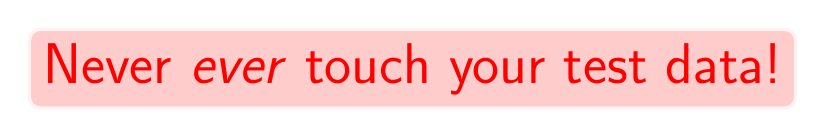
\begin{tikzpicture}[transform shape, rotate=0]
  \node [draw=Red!5, fill=Red!20, very thick, rectangle, rounded corners, inner sep=5pt, inner ysep=5pt] (box) {
    \textcolor{red}{\textsf{\huge Never \emph{ever} touch your test data!}}
  };
\end{tikzpicture}

If there is only one thing you learn from this book, let it be that.
Do not look at your test data.  Even once.  Even a tiny peek.  Once
you do that, it is not test data any more.  Yes, perhaps your
algorithm hasn't seen it.  But you have.  And you are likely a better
learner than your learning algorithm.  Consciously or otherwise, you
might make decisions based on whatever you might have seen.  Once you
look at the test data, your model's performance on it is no longer
indicative of it's performance on future unseen data.  This is simply
because future data is unseen, but your ``test'' data no longer is.

\section{Models, Parameters and Hyperparameters}

The general approach to machine learning, which captures many existing
learning algorithms, is the \concept{modeling} approach.  The idea is
that we come up with some formal model of our data.  For instance, we
might model the classification decision of a student/course pair as a
decision tree.  The choice of using a \emph{tree} to represent this
model is \emph{our choice.}  We also could have used an arithmetic
circuit or a polynomial or some other function.  The model tells us
what sort of things we can learn, and also tells us what our inductive
bias is.

For most models, there will be associated parameters.  These are the
things that we use the data to decide on.  Parameters in a decision
tree include: the specific questions we asked, the order in which we
asked them, and the classification decisions at the leaves.  The job
of our decision tree learning algorithm \FUN{DecisionTreeTrain} is to take data
and figure out a good set of parameters.

Many learning algorithms will have additional knobs that you can
adjust.  In most cases, these knobs amount to tuning the inductive
bias of the algorithm.  In the case of the decision tree, an obvious
knob that one can tune is the \concept{maximum depth} of the decision
tree.  That is, we could modify the \FUN{DecisionTreeTrain} function so that it
\emph{stops} recursing once it reaches some pre-defined maximum depth.
By playing with this depth knob, we can adjust between underfitting
(the empty tree, depth$=0$) and overfitting (the full tree,
depth$=\infty$).

\thinkaboutit{Go back to the \FUN{DecisionTreeTrain} algorithm and modify it so
  that it takes a maximum depth parameter.  This should require adding
  two lines of code and modifying three others.}

Such a knob is called a \concept{hyperparameter}.  It is so called
because it is a parameter that controls other parameters of the model.
The exact definition of hyperparameter is hard to pin down: it's one
of those things that are easier to identify than define.  However, one
of the key identifiers for hyperparameters (and the main reason that
they cause consternation) is that they cannot be naively adjusted
using the training data.

In \FUN{DecisionTreeTrain}, as in most machine learning, the learning algorithm
is essentially trying to adjust the parameters of the model so as to
minimize training error.  This suggests an idea for choosing
hyperparameters: choose them so that they minimize training error.

What is wrong with this suggestion?  Suppose that you were to treat
``maximum depth'' as a hyperparameter and tried to tune it on your
training data.  To do this, maybe you simply build a collection of
decision trees, tree$_0$, tree$_1$, tree$_2$, $\dots$, tree$_{100}$,
where tree$_d$ is a tree of maximum depth $d$.  We then computed the
training error of each of these trees and chose the ``ideal'' maximum
depth as that which minimizes training error?  Which one would it
pick?

The answer is that it would pick $d=100$.  Or, in general, it would
pick $d$ as large as possible.  Why?  Because choosing a bigger $d$
will \emph{never hurt} on the training data.  By making $d$ larger,
you are simply encouraging overfitting.  But by evaluating on the
training data, overfitting actually looks like a good idea!

An alternative idea would be to tune the maximum depth on test data.
This is promising because test data peformance is what we really want
to optimize, so tuning this knob on the test data seems like a good
idea.  That is, it won't accidentally reward overfitting.  Of course,
it breaks our cardinal rule about test data: that you should never
touch your test data.  So that idea is immediately off the table.

However, our ``test data'' wasn't magic.  We simply took our $1000$
examples, called $800$ of them ``training'' data and called the other
$200$ ``test'' data.  So instead, let's do the following.  Let's take
our original $1000$ data points, and select $700$ of them as training
data.  From the remainder, take $100$ as \concept{development
  data}\sidenote{Some people call this ``\concept{validation data}''
  or ``\concept{held-out data}.''} and the remaining $200$ as test
data.  The job of the development data is to allow us to tune
hyperparameters.  The general approach is as follows:

\begin{enumerate}
\item Split your data into $70\%$ training data, $10\%$ development
  data and $20\%$ test data.

\item For each possible setting of your hyperparameters:

\begin{enumerate}
\item Train a model using that setting of hyperparameters on the
  training data.

\item Compute this model's error rate on the development data.
\end{enumerate}

\item From the above collection of models, choose the one that
  achieved the lowest error rate on development data.

\item Evaluate that model on the test data to estimate future test
  performance.
\end{enumerate}

\thinkaboutit{In step 3, you could either choose the model (trained on
  the $70\%$ training data) that did the best on the development data.
  Or you could choose the hyperparameter settings that did best and
  \emph{retrain} the model on the $80\%$ union of training and
  development data.  Is either of these options obviously better or
  worse?}


\section{Real World Applications of Machine Learning}

Figure~\ref{fig:formal_deployml} shows a typical sequence of decisions that must be made to deploy a machine learning approach in the real world. In the left column, you can see the generic decision being made. In the right column, an example of this decision for the particular case of advertising placement on a search engine we've built.

In this sequence, (1) we have some real world goal like increasing revenue for our search engine, and decide to try to increase revenue by (2) displaying better ads. We convert this task into a machine learning problem by (3) deciding to train a classifier to predict whether a user will click on an ad or not. In order to apply machine learning, we must collect some training data; in this case, (4) we collect data by logging user interactions with the current system. We must choose what to log; (5) we choose to log the ad being displayed, the query the user entered into our search engine, and binary value showing if they clicked or not.

{
  \definecolor{lightcyan}{rgb}{0.88,1,1}
  \definecolor{lightpink}{rgb}{1,0.88,1}
  \newcolumntype{y}{>{\columncolor{lightcyan}}m{2cm}}
  \newcolumntype{z}{>{\columncolor{lightpink}}m{2cm}}
  \begin{marginfigure}[\NextFigureOffset]
    \begin{centering}
      %\includegraphics[width=1.5\textwidth]{figs/formal_deployml}
      \taburulecolor{darkblue}
      \tabulinestyle{1pt}
      \everyrow{\hline}
      \renewcommand{\arraystretch}{1.5}
      \hyphenpenalty=10000
      \exhyphenpenalty=10000
      \tabulinesep=2pt
      \begin{tabu}{|@{ }m{4mm}@{~~ }y@{~~~~}|@{}z|}
        1 & real world ~~~goal     & increase revenue        \\
        2 & real world mechanism& better ad display       \\
        3 & learning problem    & classify click-through  \\
        4 & data collection     & interaction w/ current system\\
        5 & collected data      & query, ad, click        \\
        6 & data representation & bow$^2$, $\pm$ click    \\
        7 & select model family   & decision trees, depth 20      \\
        8 & select training data   & subset from april'16    \\
        9 & train model \& hyperparams   & final decision tree     \\
       10 & predict on test data& subset from may'16      \\
       11 & evaluate error      & zero/one loss for $\pm$ click     \\
       12 & deploy! & (hope we achieve our goal)\\
      \end{tabu}
      \caption{A typical design process for a machine learning application.}
    \label{fig:formal_deployml}
    \end{centering}
  \end{marginfigure}
  \ResetNextFigure{}
}

In order to make these logs consumable by a machine learning algorithm, (6) we convert the data into input/output pairs: in this case, pairs of words from a bag-of-words representing the query and a bag-of-words representing the ad as input, and the click as a $\pm$ label. We then (7) select a model family (e.g., depth 20 decision trees), and thereby an inductive bias, for instance depth $\leq 20$ decision trees.

We're now ready to (8) select a specific subset of data to use as training data: in this case, data from April 2016. We split this into training and development and (9) learn a final decision tree, tuning the maximum depth on the development data. We can then use this decision tree to (10) make predictions on some held-out test data, in this case from the following month. We can (11) measure the overall quality of our predictor as zero/one loss (classification error) on this test data and finally (12) deploy our system.

The important thing about this sequence of steps is that \emph{in any one, things can go wrong.} That is, between any two rows of this table, we are \emph{necessarily} accumulating some additional error against our original real world goal of increasing revenue. For example, in step 5, we decided on a representation that left out many possible variables we could have logged, like time of day or season of year. By leaving out those variables, we set an explicit upper bound on how well our learned system can do.

It is often an effective strategy to run an \concept{oracle experiment}. In an oracle experiment, we assume that everything below some line can be solved perfectly, and measure how much impact that will have on a higher line. As an extreme example, before embarking on a machine learning approach to the ad display problem, we should measure something like: if our classifier were \emph{perfect}, how much more money would we make? If the number is not very high, perhaps there is some better use of our time.

Finally, although this sequence is denoted linearly, the entire process is highly interactive in practice. A large part of ``debugging'' machine learning (covered more extensively in Chapter~\ref{sec:prac} involves trying to figure out where in this sequence the biggest losses are and fixing that step. In general, it is often useful to \emph{build the stupidest thing that could possibly work}, then look at how well it's doing, and decide if and where to fix it.


\section{Further Reading}

TODO further reading


%%% Local Variables:
%%% mode: latex
%%% TeX-master: "courseml"
%%% End:
